\section{Alignment with Autonomous Vehicles}\label{sec:Alignment}

Machine learning is all up in autonomous vehicles.  It is used in the perception tasks such as segmentation of entities from sensor data.  Machine learning is also used in the decision layer of the autonomous vehicle that chooses the safest route to the destination.  Where ever there is machine learning, there is an opportunity to apply XAI.

The three use cases defined in \ref{sec:UseCases} each can be applied in the context of autonomous vehicles.  The development process of the ML systems in the vehicle can be strengthened by data provenance techniques that improve collaboration or also by using explanations to identify opportunities to improve predictive models.  Potential consumers of autonomous vehicles may feel safer when the vehicle can provide verbal explanations of the decisions that it is making.  And automakers may be inclined or, potentially, required to be able to provide explanations to legal or auditory queries for the decisions made by their autonomous systems.

There is existing research in the field of applying XAI methods in the space of autonomous vehicles, but there is much uncertainty in the scope of the relationship between these two areas.  Legal responsibilities are sometimes unclear or poorly defined for autonomous vehicle manufacturers, and the relationship between humans and AI systems is ever evolving.  It is important for researchers to forge ahead on incorporating XAI concepts in autonomous vehicles before the demand arises, not in response to it.

\subsection{Existing Research}

In one study, research subjects participated in a driving simulator in which the vehicle had a semi-autonomous feature that would initiate hard braking events in the case of an unforeseen obstacle in the path of the vehicle \cite{Koo2015}.  Researchers programmed the simulator to provide different types of verbal explanations for the hard brake events.  Survey responses from the research subjects showed that drivers had not only more positive emotional responses when more descriptive explanations were provided by the semi-autonomous system, but there was also measurably safer driving habits observed by the drivers when they received rich explanations that described not only how the vehicle was behaving but also why it was choosing those behaviors.

It is not uncommon for researchers to generate saliency maps of feature importance when doing computer vision tasks with deep neural networks.  These feature saliency maps can overlay neatly over the original image to help developers of these decision systems to identify if the responses from the neural network are behaving as expected.  Bojarski et al. developed a method of generating saliency maps called VisualBackProp \cite{DBLP:journals/corr/BojarskiCCFJMZ16} and apply it to an end-to-end autonomous driving system called PilotNet.  PilotNet can decide steering wheel angles given input images, bypassing the need for an intermediate perception phase that identifies segmented objects in images before making decisions.  VisualBackProp confirms that PilotNet is making decisions based on human-understandable features in the images, such as the boundaries of the road, lane markers, and the boundaries of other vehicles on the road (see figure \ref{fig:bojarski2017}) \cite{Bojarski2017ExplainingHA}.

\begin{figure*}
    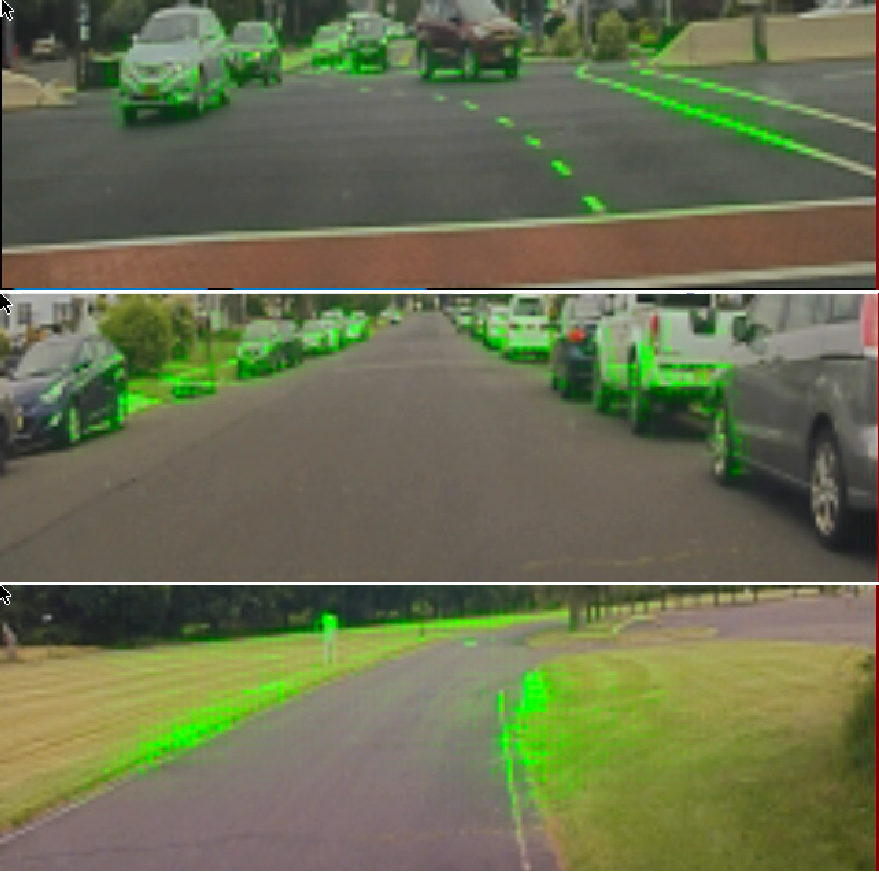
\includegraphics[width=\textwidth]{media/bojarski2017.png}
    \caption{Bojarski et al. generate saliency maps of input features in their end-to-end autonomous driving system \cite{Bojarski2017ExplainingHA}}
    \label{fig:bojarski2017}
\end{figure*}

Using visual explanations to explain the decisions of a trained model has multiple drawbacks which can be ameliorated with the emerging method of verbalization in XAI.  While saliency maps may give insight into how a model is responding to a single input, both humans and autonomous systems make decisions based on information over time.  Also, the interpretation of a visual explanation is subjective to the human audience; different observers may draw different or no insights from a single visual explanation.  Kim et al. train a LSTM neural net on a dataset of images over time accompanied by human-labeled explanations of the current driving behavior \cite{kim2018textual}.  The output layer of this trained model labels images over time with descriptive natural language of the driving behavior.  Provided as input into this verbalization model are "attention" maps of regions in the images that are identified as important features.  These regions of high and weak attention are generated from a CNN that is used to decide acceleration and course change behavior given input images.  The objective of Kim et al. of explaining a limited set of automated behavior in an autonomous vehicle via visual explanations is similar to the work of Bojarski et al \cite{Bojarski2017ExplainingHA}, but the concept is taken further by generating natural language responses to the feature relevances over time.

\subsection{Gaps and Method Alignment}

One of the most explicit use cases for applying XAI methods to the development of autonomous vehicles is in the support of researchers and engineers who are developing machine learning models, especially in the perception and decision systems of the autonomous vehicle.  In \ref{sec:UseCases} Use Cases, we identified examples of data scientists using explanations of non-intuitive, black-box ML models to improve how the models were trained and thus improve the performance of the models.  While some researchers have applied XAI to CNNs that were used in an end-to-end system to decide steering angles \cite{Bojarski2017ExplainingHA}, there was no published research found at the time of this writing on applying XAI towards the improvement of CNNs being applied in the perception system of autonomous vehicles for tasks such as object detection and object segmentation.  Deep reinforcement learning is an emerging field for training the decision systems of autonomous vehicles [citation needed], and the resulting deep q-networks (DQNs) have not been explored for explaining their decisions onto a human-interpretable domain.  

(Move this to section on legal/ethical obligations to explaining ML systems)  Besides using explanations to discover opportunities to improve models, there is no published research on the application of data provenance as a tool to assist with the ML workflow of developers of autonomous vehicles by creating 



How do we approach this section???  Potential idea:  talk about each of the three use cases in turn, addressing which items in the background can be applied to that use case that haven't been done yet.  *Demonstrate the need or value of doing so*.  Another idea:  walk through the applications of XAI in AV outlined in the second paragraph of the intro of this section

\begin{itemize}
    \item There are a couple papers about the multimodal sensors in AV, the perception/decision architecture, and a survey of decision 
    \item There are quite a few papers about establishing trust with automated systems, AI, and HCI.  Is there a gap in establishing trust that has not been addressed in previous research?
    \item Might have to put the legal/auditory use case on the back burner...way out of scope for my expertise at this time.
\end{itemize}
